% !TeX root = ../../../main.tex
\begin{figure}[htbp]
\ChThreeFloatContents
  {ch03:fig:non_adherence_level}
  {\caption{Distribution of Average Continuous Non-Adherence across Patients. (a) All Patients, (b) Patients prescribed with Injectable Medications (at least once in their trajectory), (c) Patients prescribed with Non-Injectable Medications. The x-axis shows the number of days in a month that a patient goes non-adherent on average. Non-coverage of less than 10 days in month is considered \textcolor{blue}{Adherent}, and for more than 10 days is considered \textcolor{red}{Non-Adherent} in our setup.}}
  {%
    \subfigure[All Patients]{\label{ch03:fig:non_adherence_all}%
      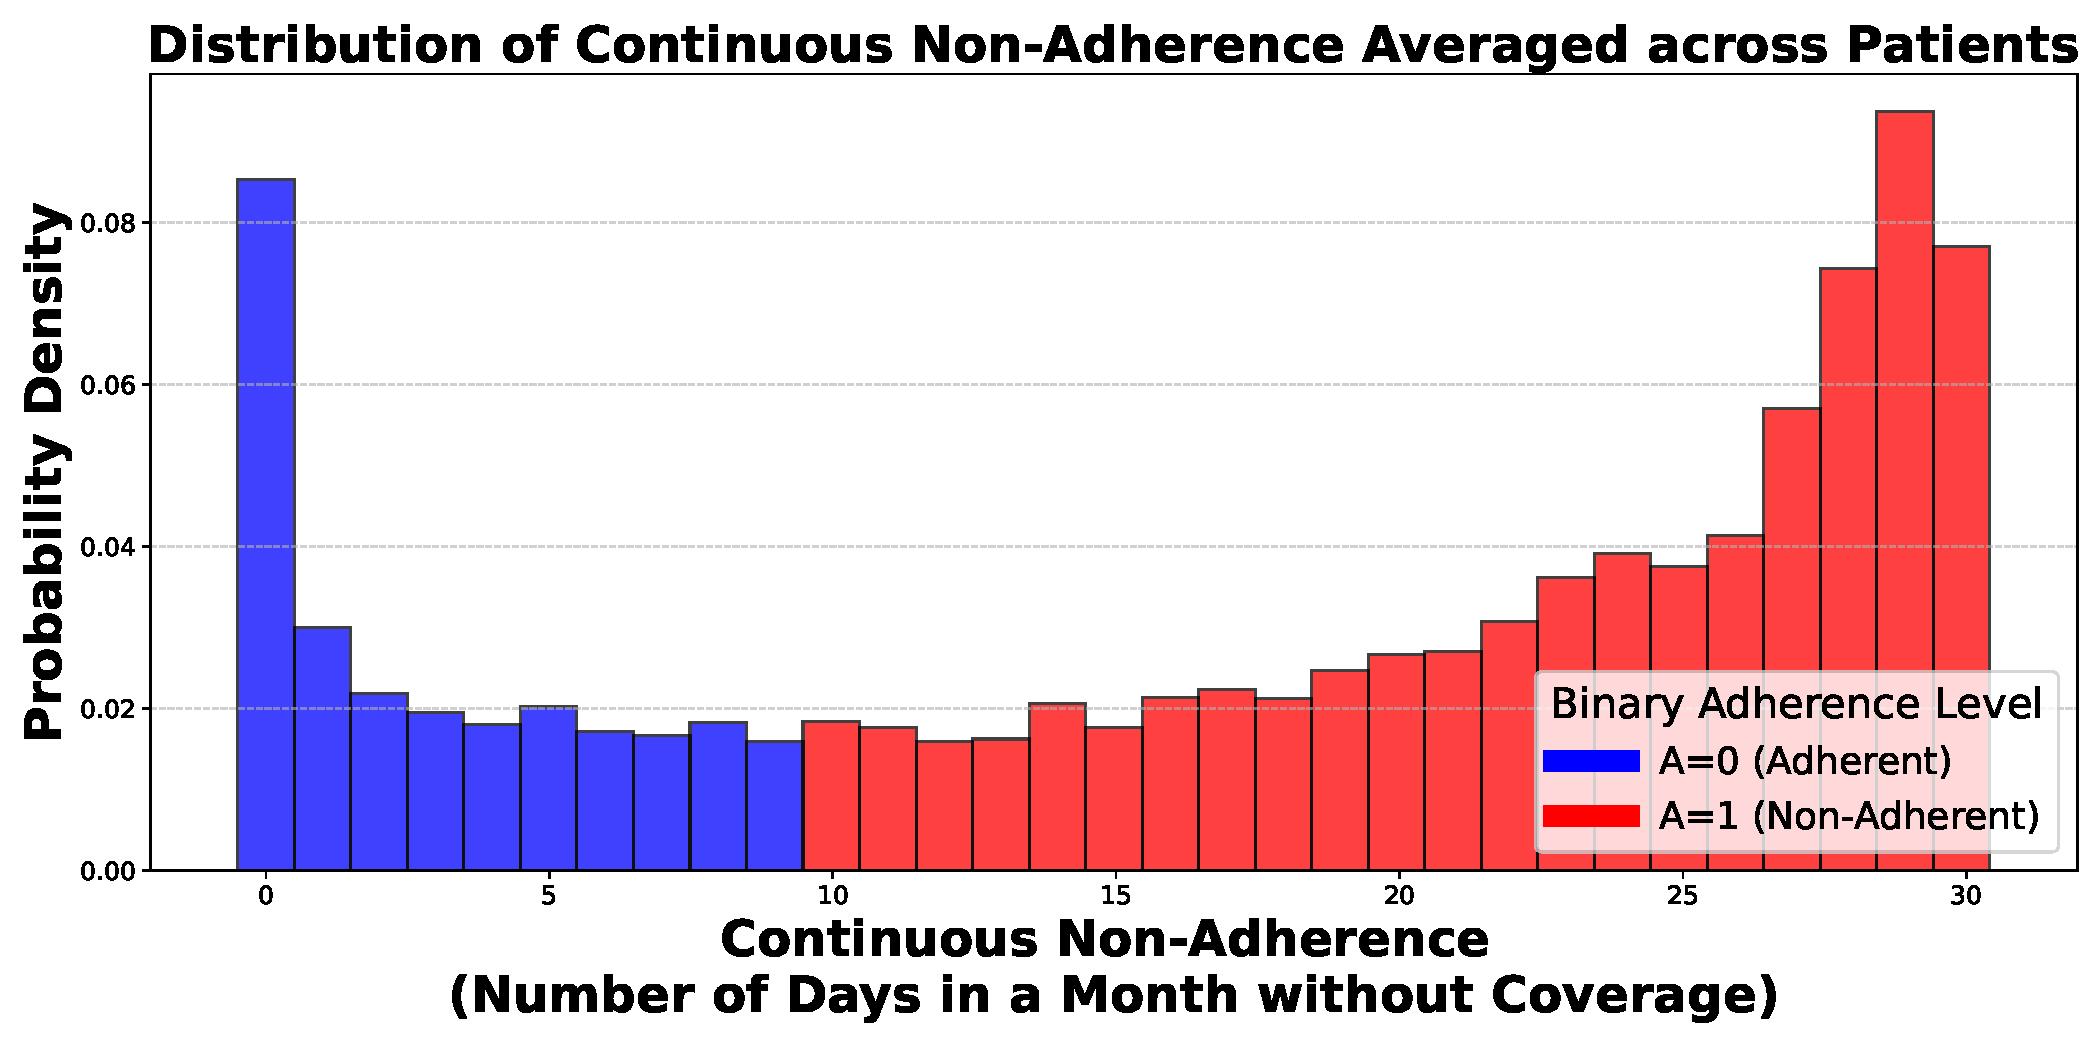
\includegraphics[width=\linewidth]{Appendices/appendix-ch03/images/Non_Adherence_Levels/distribution_of_continuous_non-adherence_for_all_patients.pdf}}%
    \\
    \subfigure[Patients with Injectable Medication]{\label{ch03:fig:non_adherence_injectable}%
      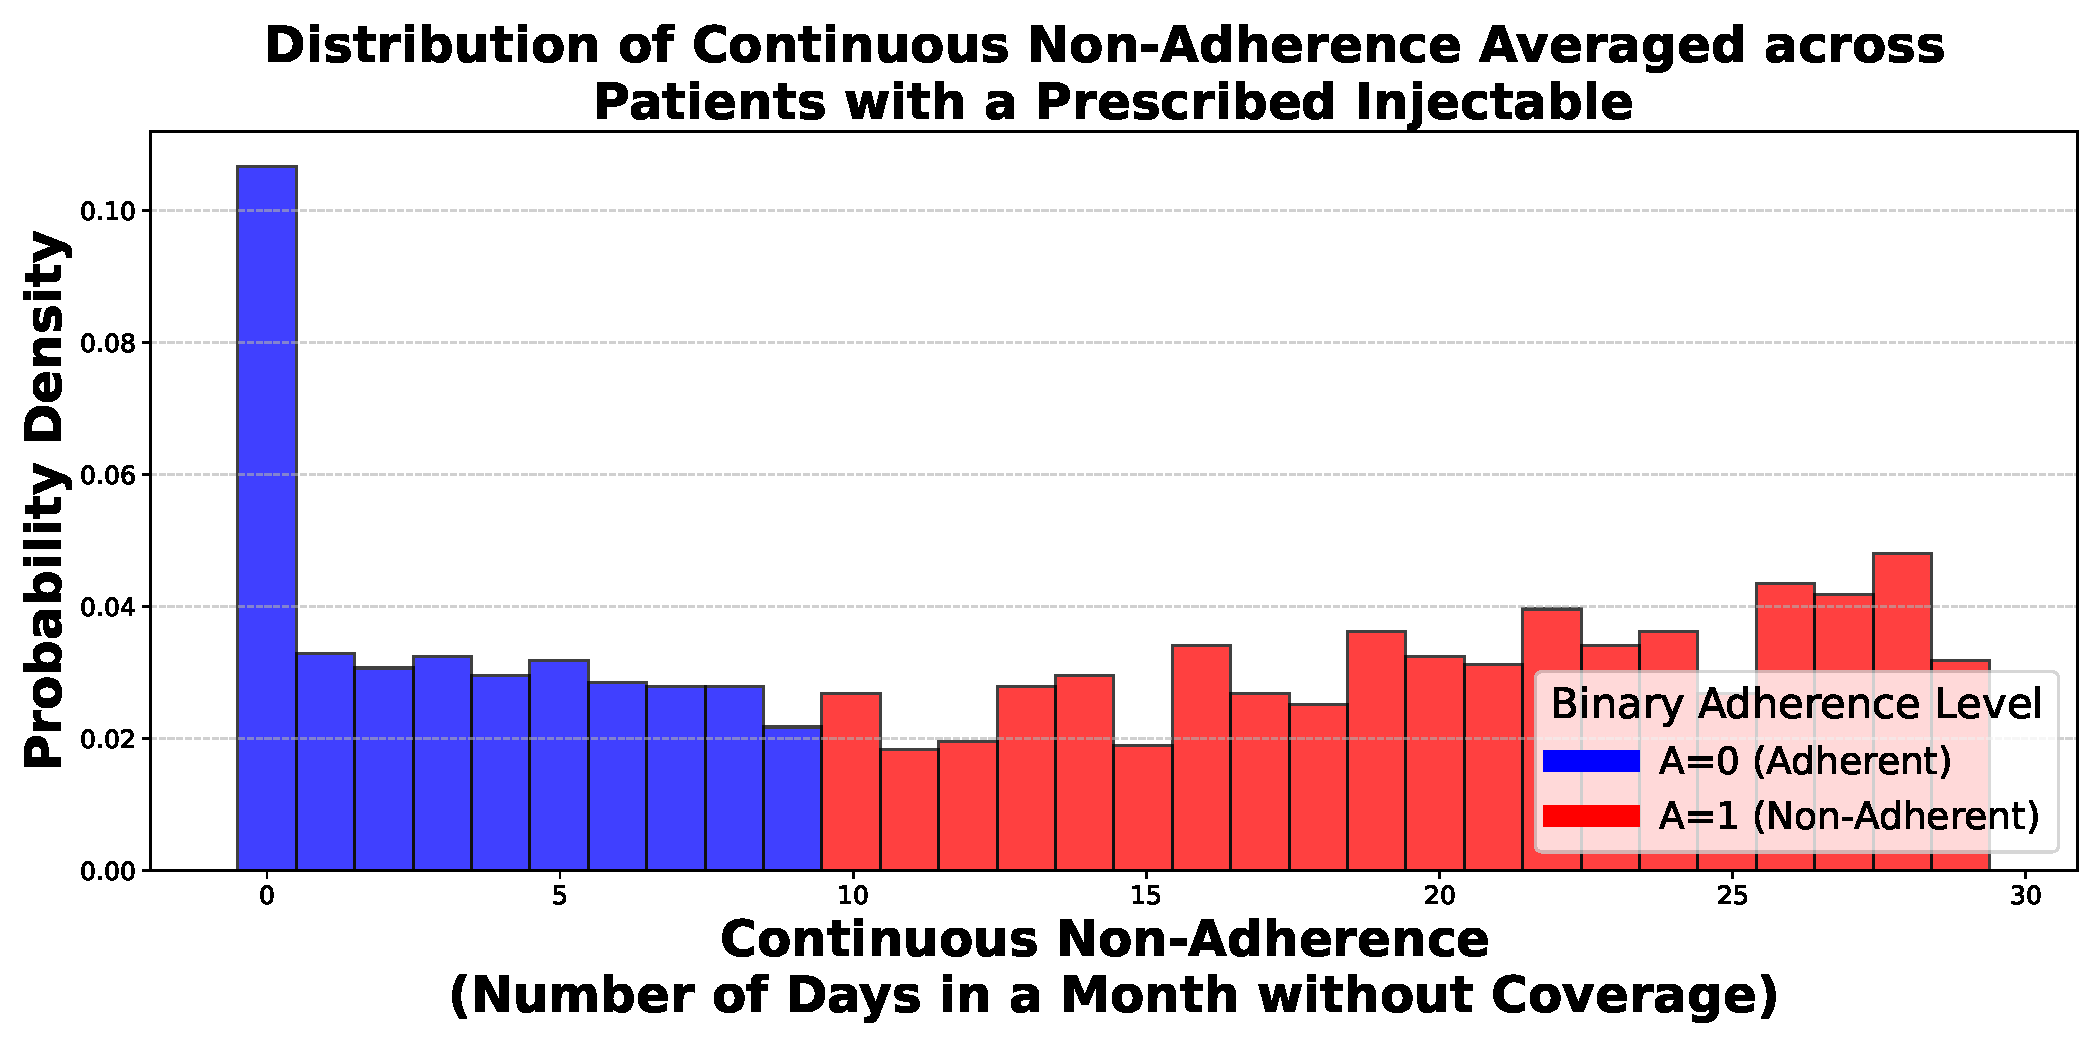
\includegraphics[width=\linewidth]{Appendices/appendix-ch03/images/Non_Adherence_Levels/distribution_of_continuous_non_adherence_for_patients_with_injectables.pdf}}%
    \\
    \subfigure[Patients with Non-Injectable Medication]{\label{ch03:fig:non_adherence_non_injectable}%
      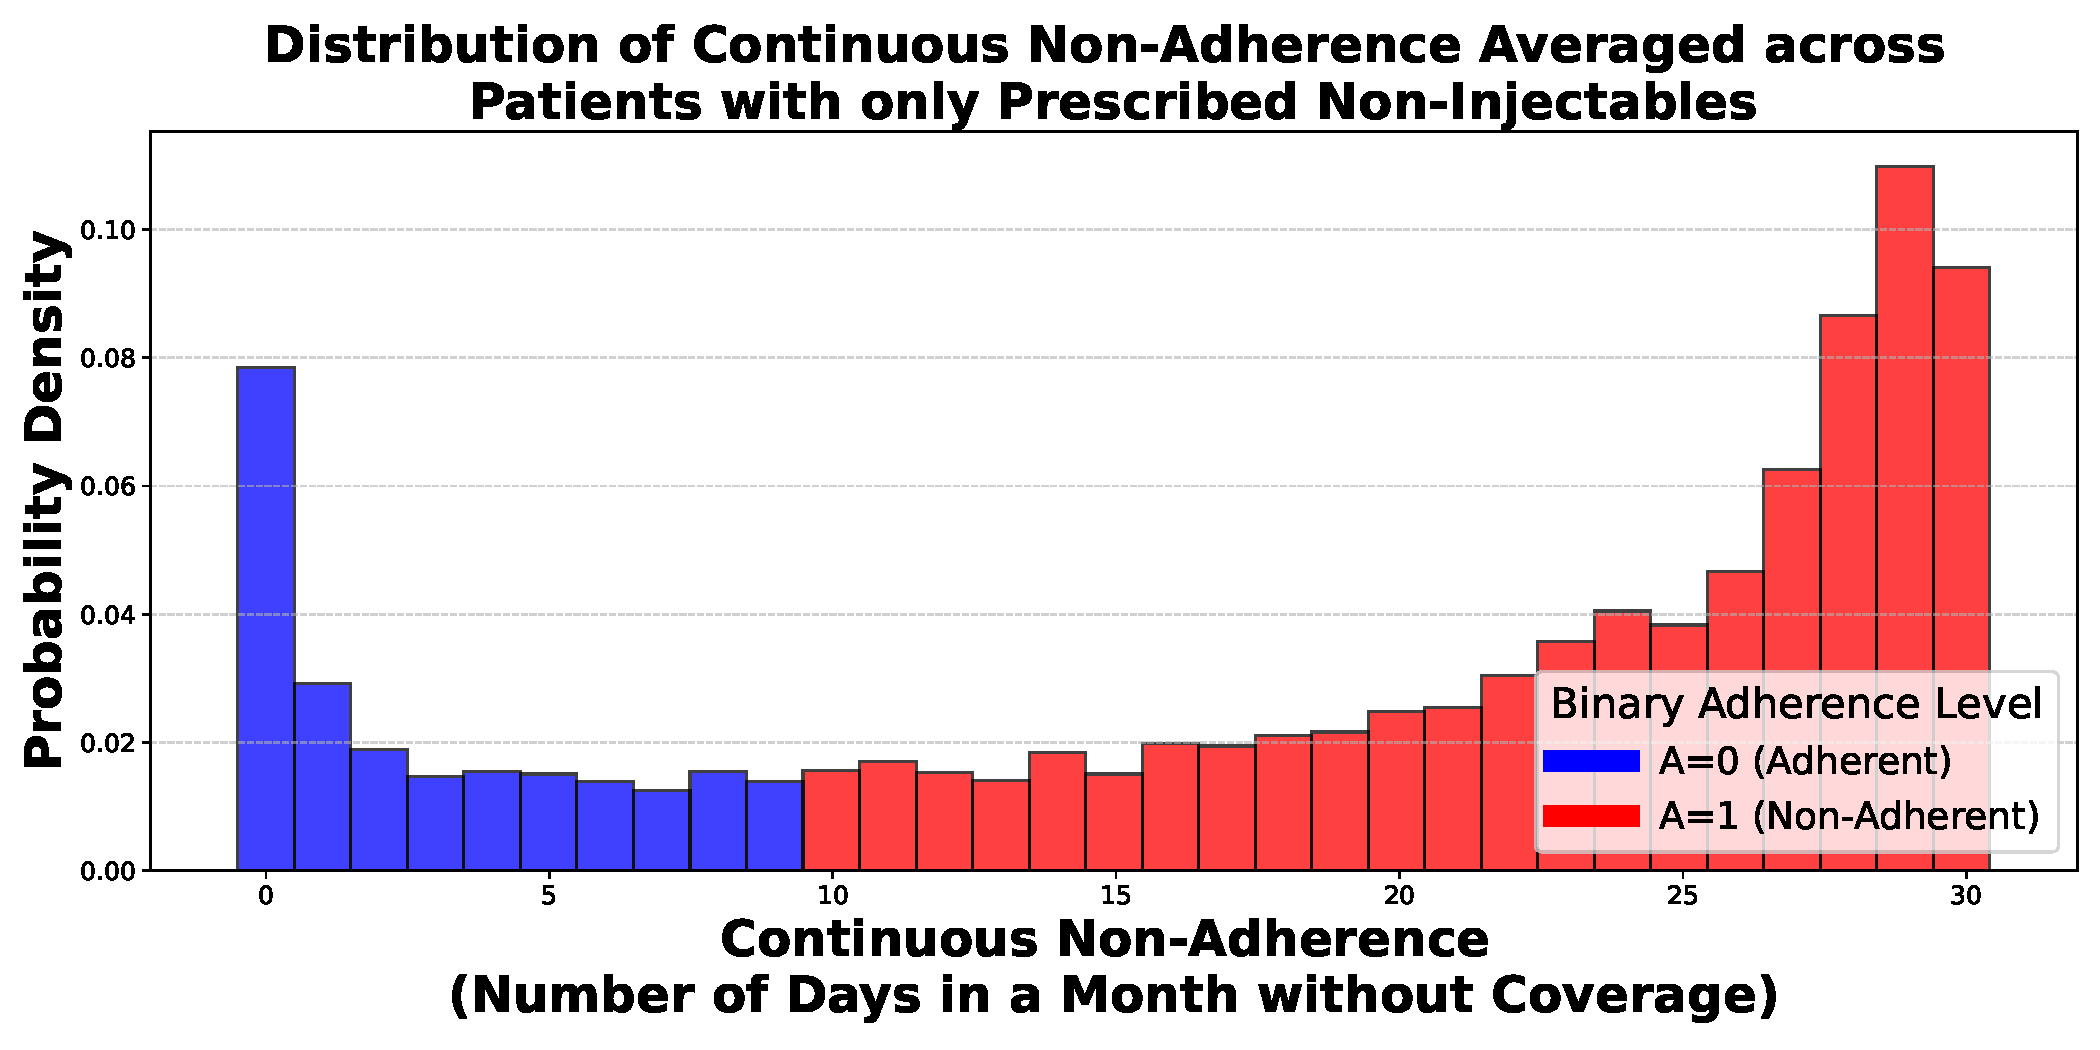
\includegraphics[width=\linewidth]{Appendices/appendix-ch03/images/Non_Adherence_Levels/distribution_of_continuous_non_adherence_for_patients_with_non-injectables.pdf}}%
  }
\end{figure}